% Options for packages loaded elsewhere
\PassOptionsToPackage{unicode}{hyperref}
\PassOptionsToPackage{hyphens}{url}
\PassOptionsToPackage{dvipsnames,svgnames,x11names}{xcolor}
%
\documentclass[
  letterpaper,
]{scrreprt}

\usepackage{amsmath,amssymb}
\usepackage{iftex}
\ifPDFTeX
  \usepackage[T1]{fontenc}
  \usepackage[utf8]{inputenc}
  \usepackage{textcomp} % provide euro and other symbols
\else % if luatex or xetex
  \usepackage{unicode-math}
  \defaultfontfeatures{Scale=MatchLowercase}
  \defaultfontfeatures[\rmfamily]{Ligatures=TeX,Scale=1}
\fi
\usepackage{lmodern}
\ifPDFTeX\else  
    % xetex/luatex font selection
  \setmainfont[]{TeX Gyre Pagella}
\fi
% Use upquote if available, for straight quotes in verbatim environments
\IfFileExists{upquote.sty}{\usepackage{upquote}}{}
\IfFileExists{microtype.sty}{% use microtype if available
  \usepackage[]{microtype}
  \UseMicrotypeSet[protrusion]{basicmath} % disable protrusion for tt fonts
}{}
\makeatletter
\@ifundefined{KOMAClassName}{% if non-KOMA class
  \IfFileExists{parskip.sty}{%
    \usepackage{parskip}
  }{% else
    \setlength{\parindent}{0pt}
    \setlength{\parskip}{6pt plus 2pt minus 1pt}}
}{% if KOMA class
  \KOMAoptions{parskip=half}}
\makeatother
\usepackage{xcolor}
\setlength{\emergencystretch}{3em} % prevent overfull lines
\setcounter{secnumdepth}{5}
% Make \paragraph and \subparagraph free-standing
\ifx\paragraph\undefined\else
  \let\oldparagraph\paragraph
  \renewcommand{\paragraph}[1]{\oldparagraph{#1}\mbox{}}
\fi
\ifx\subparagraph\undefined\else
  \let\oldsubparagraph\subparagraph
  \renewcommand{\subparagraph}[1]{\oldsubparagraph{#1}\mbox{}}
\fi


\providecommand{\tightlist}{%
  \setlength{\itemsep}{0pt}\setlength{\parskip}{0pt}}\usepackage{longtable,booktabs,array}
\usepackage{calc} % for calculating minipage widths
% Correct order of tables after \paragraph or \subparagraph
\usepackage{etoolbox}
\makeatletter
\patchcmd\longtable{\par}{\if@noskipsec\mbox{}\fi\par}{}{}
\makeatother
% Allow footnotes in longtable head/foot
\IfFileExists{footnotehyper.sty}{\usepackage{footnotehyper}}{\usepackage{footnote}}
\makesavenoteenv{longtable}
\usepackage{graphicx}
\makeatletter
\def\maxwidth{\ifdim\Gin@nat@width>\linewidth\linewidth\else\Gin@nat@width\fi}
\def\maxheight{\ifdim\Gin@nat@height>\textheight\textheight\else\Gin@nat@height\fi}
\makeatother
% Scale images if necessary, so that they will not overflow the page
% margins by default, and it is still possible to overwrite the defaults
% using explicit options in \includegraphics[width, height, ...]{}
\setkeys{Gin}{width=\maxwidth,height=\maxheight,keepaspectratio}
% Set default figure placement to htbp
\makeatletter
\def\fps@figure{htbp}
\makeatother
% definitions for citeproc citations
\NewDocumentCommand\citeproctext{}{}
\NewDocumentCommand\citeproc{mm}{%
  \begingroup\def\citeproctext{#2}\cite{#1}\endgroup}
\makeatletter
 % allow citations to break across lines
 \let\@cite@ofmt\@firstofone
 % avoid brackets around text for \cite:
 \def\@biblabel#1{}
 \def\@cite#1#2{{#1\if@tempswa , #2\fi}}
\makeatother
\newlength{\cslhangindent}
\setlength{\cslhangindent}{1.5em}
\newlength{\csllabelwidth}
\setlength{\csllabelwidth}{3em}
\newenvironment{CSLReferences}[2] % #1 hanging-indent, #2 entry-spacing
 {\begin{list}{}{%
  \setlength{\itemindent}{0pt}
  \setlength{\leftmargin}{0pt}
  \setlength{\parsep}{0pt}
  % turn on hanging indent if param 1 is 1
  \ifodd #1
   \setlength{\leftmargin}{\cslhangindent}
   \setlength{\itemindent}{-1\cslhangindent}
  \fi
  % set entry spacing
  \setlength{\itemsep}{#2\baselineskip}}}
 {\end{list}}
\usepackage{calc}
\newcommand{\CSLBlock}[1]{\hfill\break\parbox[t]{\linewidth}{\strut\ignorespaces#1\strut}}
\newcommand{\CSLLeftMargin}[1]{\parbox[t]{\csllabelwidth}{\strut#1\strut}}
\newcommand{\CSLRightInline}[1]{\parbox[t]{\linewidth - \csllabelwidth}{\strut#1\strut}}
\newcommand{\CSLIndent}[1]{\hspace{\cslhangindent}#1}


% Wird für die Tabelle im Titelblatt der Experten verwendet:
% Array
\usepackage{array}
% Neue Definition für Tabelleneinträge
% linksbündig mit Breitenangabe
\newcolumntype{L}[1]{>{\raggedright\arraybackslash}p{#1}} 
% zentriert mit Breitenangabe
\newcolumntype{C}[1]{>{\centering\arraybackslash}p{#1}} 
% rechtsbündig mit Breitenangabe
\newcolumntype{R}[1]{>{\raggedleft\arraybackslash}p{#1}} 

\usepackage[a4paper, margin=3cm]{geometry}

% Titles take mainfont
\addtokomafont{disposition}{\rmfamily}





\makeatletter
\@ifpackageloaded{bookmark}{}{\usepackage{bookmark}}
\makeatother
\makeatletter
\@ifpackageloaded{caption}{}{\usepackage{caption}}
\AtBeginDocument{%
\ifdefined\contentsname
  \renewcommand*\contentsname{Inhaltsverzeichnis}
\else
  \newcommand\contentsname{Inhaltsverzeichnis}
\fi
\ifdefined\listfigurename
  \renewcommand*\listfigurename{Abbildungsverzeichnis}
\else
  \newcommand\listfigurename{Abbildungsverzeichnis}
\fi
\ifdefined\listtablename
  \renewcommand*\listtablename{Tabellenverzeichnis}
\else
  \newcommand\listtablename{Tabellenverzeichnis}
\fi
\ifdefined\figurename
  \renewcommand*\figurename{Abbildung}
\else
  \newcommand\figurename{Abbildung}
\fi
\ifdefined\tablename
  \renewcommand*\tablename{Tabelle}
\else
  \newcommand\tablename{Tabelle}
\fi
}
\@ifpackageloaded{float}{}{\usepackage{float}}
\floatstyle{ruled}
\@ifundefined{c@chapter}{\newfloat{codelisting}{h}{lop}}{\newfloat{codelisting}{h}{lop}[chapter]}
\floatname{codelisting}{Listing}
\newcommand*\listoflistings{\listof{codelisting}{Listingverzeichnis}}
\makeatother
\makeatletter
\makeatother
\makeatletter
\@ifpackageloaded{caption}{}{\usepackage{caption}}
\@ifpackageloaded{subcaption}{}{\usepackage{subcaption}}
\makeatother
\ifLuaTeX
\usepackage[bidi=basic]{babel}
\else
\usepackage[bidi=default]{babel}
\fi
\babelprovide[main,import]{ngerman}
\ifPDFTeX
\else
\babelfont{rm}[]{TeX Gyre Pagella}
\fi
% get rid of language-specific shorthands (see #6817):
\let\LanguageShortHands\languageshorthands
\def\languageshorthands#1{}
\ifLuaTeX
  \usepackage{selnolig}  % disable illegal ligatures
\fi
\usepackage{bookmark}

\IfFileExists{xurl.sty}{\usepackage{xurl}}{} % add URL line breaks if available
\urlstyle{same} % disable monospaced font for URLs
\hypersetup{
  pdftitle={Tragverhalten von Stahlbetontragwerken},
  pdfauthor={Pascal Gitz},
  pdflang={de},
  colorlinks=true,
  linkcolor={Black},
  filecolor={Maroon},
  citecolor={Blue},
  urlcolor={Blue},
  pdfcreator={LaTeX via pandoc}}

% TITELBLATT, VERSIONSTABELLE UND SELBSTSTÄNDIGKEITSERKLÄRUNG
%--------------------------------------------------------------------------------------------------------------------


\titlehead{
\includegraphics[height=0.5cm]{../imgs/logos/logo-mse}\hfill
\includegraphics[height=0.5cm]{../imgs/logos/logo-hslu-en-col} \\ }
\subject{MASTER OF SCIENCE IN ENGINEERING\\Vertiefungsmodul II}
\title{Tragverhalten von Stahlbetontragwerken}

\subtitle
{Ansätze zur Modellierung}

%\thanks{
%Version 1.0
%\hfill \today
%\hfill Hun}


\date{\large Horw, Freitag, 14. Juni 2024}
\author{Pascal Gitz}

\publishers{
	\begin{table}[H]
		\centering
		\begin{tabular}{L{2cm} L{6cm}}
			Advisor: & Prof. FH, Dr. Daniel Heinzmann \\
			Experte: & Dr. Thomas Jäger \\
		\end{tabular}
	\end{table}
}
\begin{document}
\maketitle


Hiermit erkläre ich, dass ich die vorliegende Arbeit selbstständig angefertigt und keine anderen als die angegebenen Hilfsmittel verwendet habe. Sämtliche verwendeten Textausschnitte, Zitate oder Inhalte anderer Verfasser wurden ausdrücklich als solche gekennzeichnet.\\%
%
\\%
%
Horw, 14. Juni 2024 \hfill Pascal Gitz%

\vfill
%\begin{tabular}[h]{llcr} 
    %*Version 2.0 & - Definitives Exemplar & \today & MK \\ 
    %*Version 1.0 & - Prüfungsexemplar & 22. Januar 2021 & MK \\ 
%\end{tabular}\\

% Version 2.0 - Definitives Exemplar \hfill \today \quad \quad \quad \quad \quad MK\\
Version 1.0 - Prüfungsexemplar \hfill 14. Juni 2024 \quad \quad \quad \quad \quad PG\\
Version 0.9 - Entwurf \hfill 07. Juni 2024 \quad \quad \quad \quad \quad PG\\

\newpage

\chapter*{Kurzfassung}

-

\renewcommand*\contentsname{Inhaltsverzeichnis}
{
\hypersetup{linkcolor=}
\setcounter{tocdepth}{1}
\tableofcontents
}
\listoffigures
\listoftables
\bookmarksetup{startatroot}

\chapter{Einleitung}\label{einleitung}

\begin{itemize}
\tightlist
\item
\end{itemize}

\bookmarksetup{startatroot}

\chapter{Modellvorstellung}\label{sec-modellvorstellung}

In der Vorarbeit {[}\citeproc{ref-gitz_ansatze_2024}{1}{]} zu dieser
Arbeit wurde mittels der numerischen Integration der Krümmung das
nicht-lineare Verformungsverhalten von unterschiedlichen Versuchen
zufriedenstellend abgebildet. Um das Vorgehen auf statisch unbestimmte
Systeme zu erweitern, sowie in der Geometrie der Systeme die nötige
Flexiblität zu erhalten, wird versucht, basierend auf dem angewendeten
Berechnungsansatz, ein Stabstatikmodell zu erstellen. Die
Abbildung~\ref{fig-modell_drehfeder} zeigt eine Modellierung eines
einfachen Balkens. Dabei sind biege- und schubsteife Stäbe mit
Drehfedern gekoppelt. Dies führt dazu, dass sämtliche Deformationen des
Systems aus den Federverbindungen erfolgen.

\begin{figure}[H]

\centering{

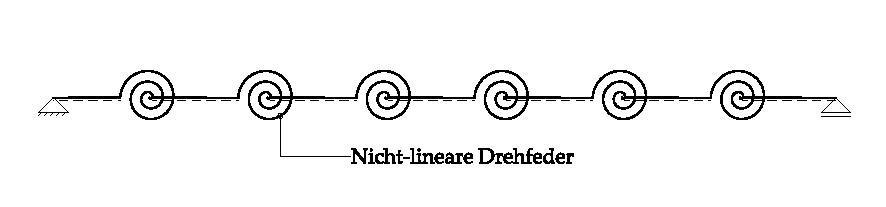
\includegraphics{index_files/mediabag/../imgs/Modell_Drehfeder.pdf}

}

\caption{\label{fig-modell_drehfeder}Modellierung als biegesteife Stäbe
gekoppelt mit Drehfedern}

\end{figure}%

Mit der Wahl der entsprechenden Federcharakteristiken stellen sich so
die passenden Resultate ein. Die Anwendung des Modells an
experimentellen Versuchen wird in den folgenden Kapiteln aufgegriffen.
Es lässt sich vorweggreifen, dass die Wahl der Federcharakteristik die
Krux des Systems darstellt.

Alternativ zur Modellierung mittels Drehfedern lässt sich das Verhalten
der Drehfeder mit einem Wegfederpaar abbilden. Dies erlaubt eine
Modellierung mittels den nicht-linearen Fachwerksstäben der Software
Statik-9 der Cubus AG. Dieser Ansatz wird lediglich im
Einführungsbeispiel berücksichtigt.

\begin{figure}[H]

\centering{

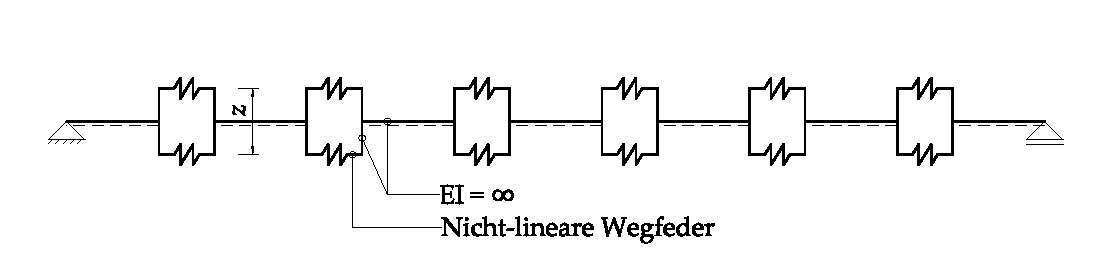
\includegraphics{index_files/mediabag/../imgs/Modell_Wegfeder.pdf}

}

\caption{\label{fig-modell_wegfeder}Modellierung als biegesteife Stäbe
gekoppelt mit einem Wegfederpaar}

\end{figure}%

\bookmarksetup{startatroot}

\chapter{Einführungsbeispiel}\label{einfuxfchrungsbeispiel}

Das Einführungsbeispiel verfolgt das Ziel das Modellverhalten zu
plausibilisieren. Die Eingabe der nicht-linearen Parameter in der
Statiksoftware liegt im Vordergrund.

Es werden die Verformungen des fiktiven Beispiels von Hand mittels der
Arbeitsgleichung, sowie numerisch mit der Stabstatik-Software ermittelt.
Das statische System ist in Abbildung~\ref{fig-kragarm-feder}
aufgezeigt. Das Beispiel ist mit einer Drehfeder versehen, welche eine
nicht-lineare Federcharakteristik aufweist. Es werden zwei Laststufen
betrachtet. Diese sind entsprechend gewählt, dass das nicht-lineare
Verhalten der Drehfeder zu tragen kommt.

\begin{figure}[H]

\centering{

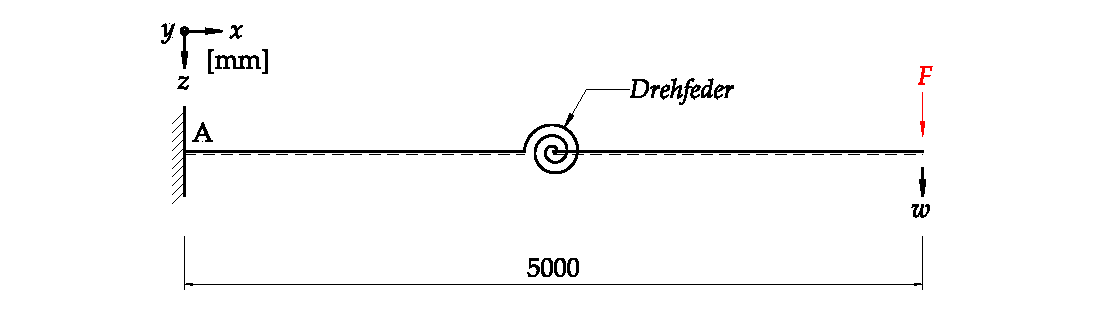
\includegraphics{index_files/mediabag/../imgs/Kragarm_system_Feder.pdf}

}

\caption{\label{fig-kragarm-feder}Statisches System des Kragarms}

\end{figure}%

Die folgenden Parameter fliessen in die Berechnungen ein. Beschrieben
sind die Abmessungen und Materialeigenschaften, sowie die beiden
Laststufen \(F_1\) und \(F_2\), wie auch die Federsteifigkeiten
\(k_{\varphi1}\) und \(k_{\varphi2}\).

$$
\begin{aligned}
E &= 10000.0\ \frac{\mathrm{N}}{\mathrm{mm}^{2}} \; 
 &F_{1} &= -10000.0\ \mathrm{N} \; 
 &F_{2} &= -21500.0\ \mathrm{N} \; 
\\[12pt]
 h &= 400.0\ \mathrm{mm} \; 
 &k_{\phi_{1}} &= 100000.0\ \frac{\mathrm{N} \cdot \mathrm{m}}{\mathrm{rad}} \; 
 &k_{\phi_{2}} &= 10000.0\ \frac{\mathrm{N} \cdot \mathrm{m}}{\mathrm{rad}} \; 
\\[12pt]
 l_{Kragarm} &= 5.0\ \mathrm{m} \; 
 &z &= 400.0\ \mathrm{mm} \; 
 &b &= 200.0\ \mathrm{mm} \; 
\\[12pt]
\end{aligned}
$$

Der Rechteckquerschnitt ist in Abbildung~\ref{fig-qs-kragarm}
aufgezeigt, dieser gilt für den gesamten Kragarm.

\begin{figure}[H]

\centering{

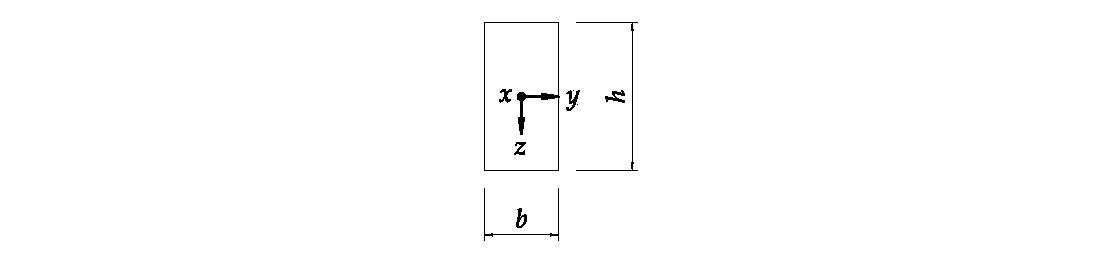
\includegraphics{index_files/mediabag/../imgs/Kragarm_querschnitt.pdf}

}

\caption{\label{fig-qs-kragarm}Fiktiver Querschnitt des Kragarms mit
durchwegs linear-elastischem Materialverhalten}

\end{figure}%

Die Entsprechende Federcharakteristik ist in
Abbildung~\ref{fig-springcharacteristic} zu sehen. Das Bilineare
Verhalten gilt für positive und negative Biegemomente um die
\(Y\)-Achse.

\begin{figure}[H]

\centering{

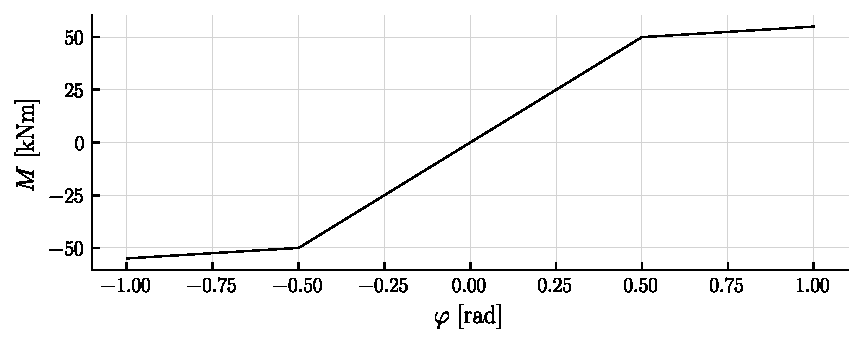
\includegraphics{index_files/mediabag/04_Kragarm_files/figure-pdf/fig-springcharacteristic-output-1.pdf}

}

\caption{\label{fig-springcharacteristic}Charakteristik der Drehfeder}

\end{figure}%

\section{Biegeverformung}\label{biegeverformung}

Zunächst werden die Biegeverformungen mittels der Differentialgleichung
für reine Biegeträger ermittelt. Dabei wird die Drehfeder
vernachlässigt. Das statische System, gezeigt in
Abbildung~\ref{fig-kragarm-sys} führt zu den Zustandslinien der
Schnittgrössen in der Abbildung~\ref{fig-skkragarmreal}.

\begin{figure}[H]

\centering{

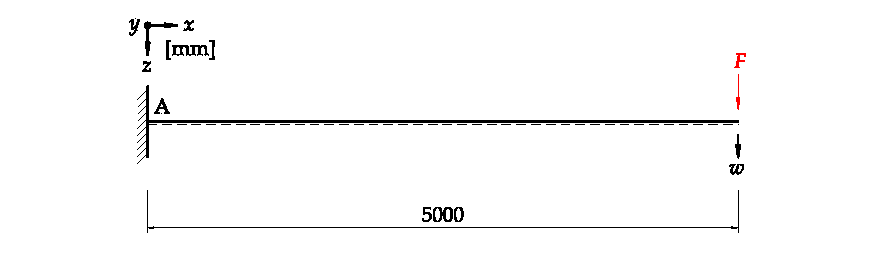
\includegraphics{index_files/mediabag/../imgs/Kragarm_System.pdf}

}

\caption{\label{fig-kragarm-sys}Statisches System des Kragarms}

\end{figure}%

\begin{figure}[H]

\centering{

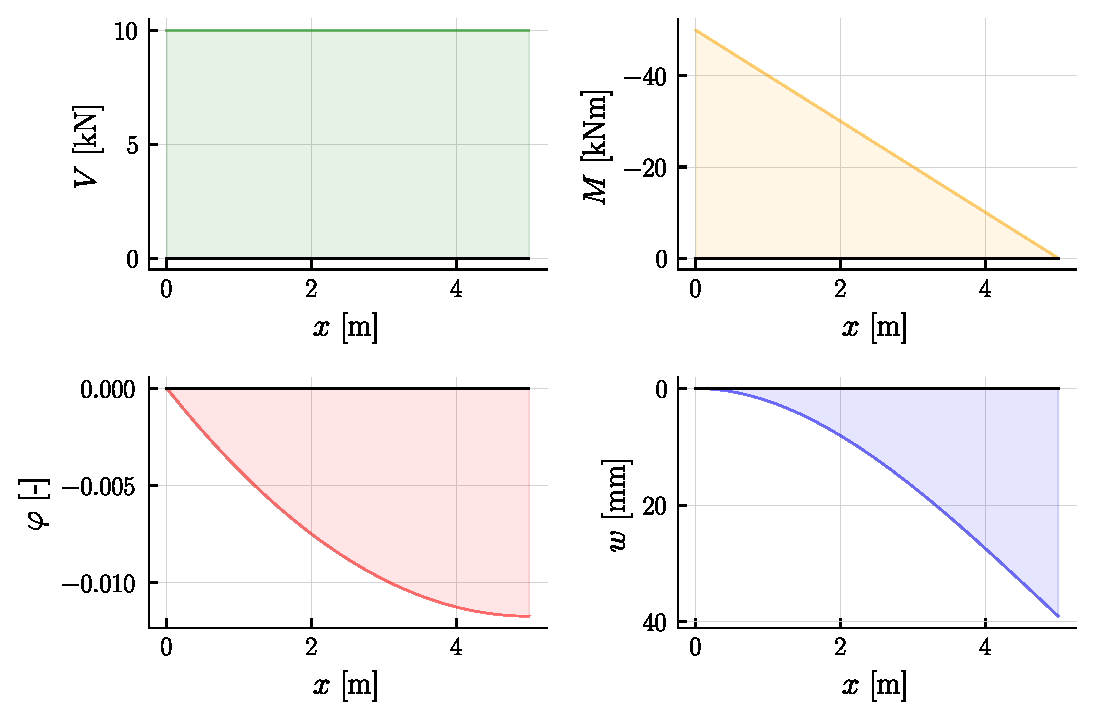
\includegraphics{index_files/mediabag/04_Kragarm_files/figure-pdf/fig-skkragarmreal-output-1.pdf}

}

\caption{\label{fig-skkragarmreal}Schnittkräfte des Systems aus
Abbildung~\ref{fig-kragarm-sys} für die Last \(F_1\)}

\end{figure}%

Die maximale Verformung am Endpunkt des Kragarms beträgt:

$$
\begin{aligned}
w_{bendingF1} &= 39.1\ \mathrm{mm} \;
\end{aligned}
$$

Das analoge Vorgehen führt für die Laststufe \(F_2\) zu den
Zustandslinien der Schnittgrössen gemäss der
Abbildung~\ref{fig-skkragarmreal_high}.

\begin{figure}[H]

\centering{

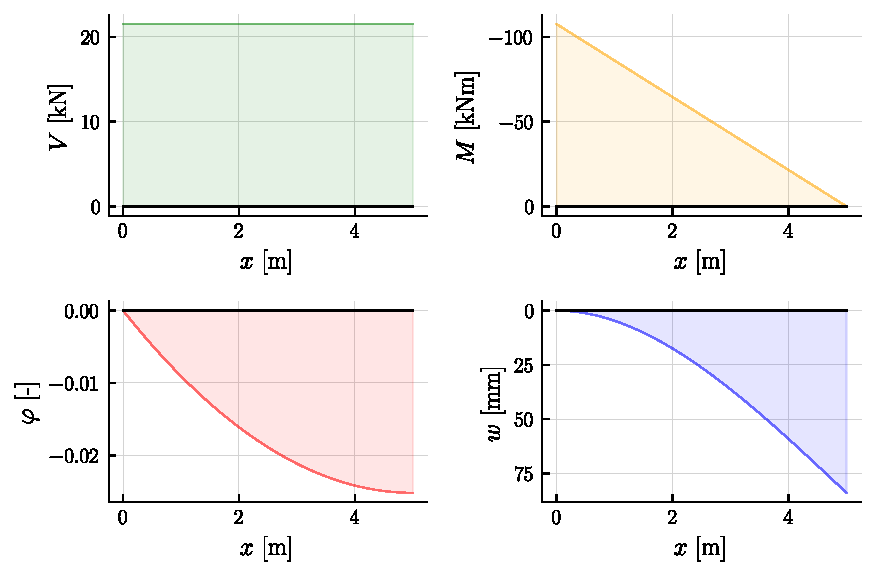
\includegraphics{index_files/mediabag/04_Kragarm_files/figure-pdf/fig-skkragarmreal_high-output-1.pdf}

}

\caption{\label{fig-skkragarmreal_high}Schnittkräfte des Systems aus
Abbildung~\ref{fig-kragarm-sys} für die Last \(F2\)}

\end{figure}%

Da ein durchwegs linear-elastisches Biegeverhalten vorausgesetzt wird,
entspricht der Faktor der Erhöhung des Verformung dem Quotient der
beiden Laststufen.

\[
\frac{w_{1,Bending,F2}}{w_{1,Bending,F1}} = \frac{F_2}{F_1}
\]

Dabei entspricht die maximale Biegeverformung am Ende des Kragarms:

$$
\begin{aligned}
w_{bendingF2} &= 84.0\ \mathrm{mm} \;
\end{aligned}
$$

\section{Verformung der Drehfeder}\label{verformung-der-drehfeder}

Zur Bestimmung der Verformung am Ende des Kragarms des Systems mit der
Drehfeder wird die Arbeitsgleichung angewendet. Dazu wird an einem
virtuellen System eine Einzellast eingeführt, an der Stelle an dem die
Verformung bestimmt werden soll. Dargestellt ist dies in
Abbildung~\ref{fig-kragarm-sys-virtuell}.

\begin{figure}[H]

\centering{

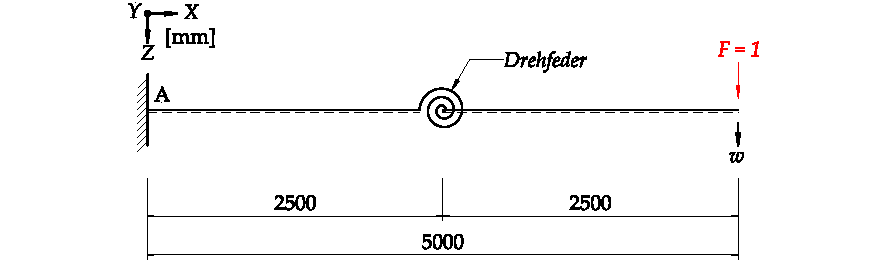
\includegraphics{index_files/mediabag/../imgs/Kragarm_system_feder_virtuell.pdf}

}

\caption{\label{fig-kragarm-sys-virtuell}Statisches System des Kragarms
im virtuellen Kräftezustand}

\end{figure}%

Die entsprechenden Verläufe der Querkraft und des Biegemoments zeigt die
Abbildung~\ref{fig-sk-kragarm-virtuell} für das virtuelle System.

\begin{figure}[H]

\centering{

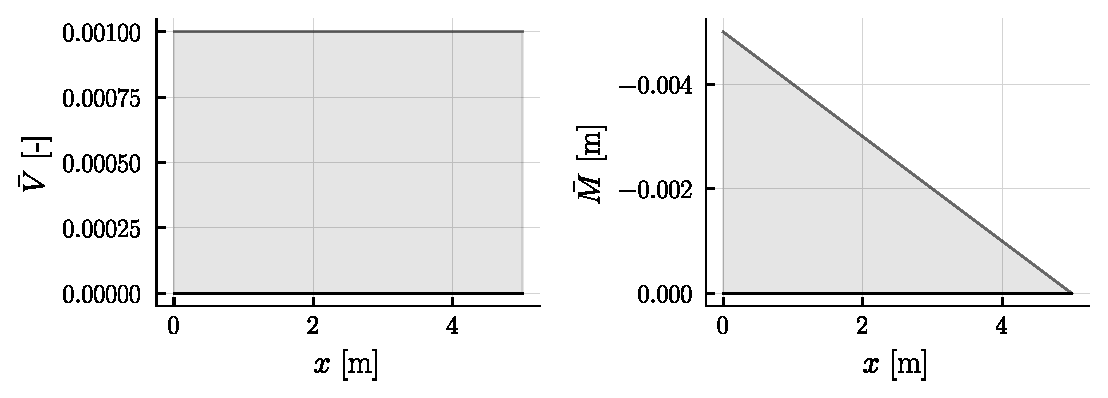
\includegraphics{index_files/mediabag/04_Kragarm_files/figure-pdf/fig-sk-kragarm-virtuell-output-1.pdf}

}

\caption{\label{fig-sk-kragarm-virtuell}Schnittkräfte des virtuellen
Systems aus Abbildung~\ref{fig-kragarm-sys-virtuell}}

\end{figure}%

Die Verformung der Drehfeder kann abschliessend mit der folgenden
Gleichung bestimmt werden.

\[
w_{Spring} = \bar{M} \frac{M}{k_\varphi} = \bar{M} \varphi
\]

Die Verdrehung lässt sich aus der Federcharakteristik mit dem
Biegemoment an der Stelle der Drehfeder bestimmen. Die
Abbildung~\ref{fig-feder-force} zeigt die Position der Laststufen im
Diagramm.

\begin{figure}[H]

\centering{

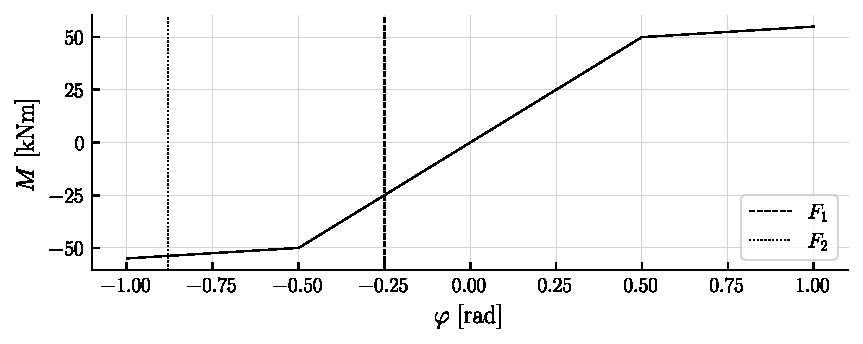
\includegraphics{index_files/mediabag/04_Kragarm_files/figure-pdf/fig-feder-force-output-1.pdf}

}

\caption{\label{fig-feder-force}Charakteristik der Drehfeder mit
Bestimmung der Verdrehung anhand der Laststufen}

\end{figure}%

Angewendet auf das System der Abbildung~\ref{fig-kragarm-feder} folgen
für die beiden Laststufen die Deformationen der Drehfeder zu:

$$
\begin{aligned}
w_{spring_{F1}} &= 625.0\ \mathrm{mm} \; 
 &w_{spring_{F2}} &= 2201.3\ \mathrm{mm} \;
\end{aligned}
$$

Dazu gilt es den Anteil aus der Biegeverformung zu addieren. Die totale
Verformung folgt zu:

$$
\begin{aligned}
w_{tot_{F1}} &= w_{spring_{F1}} + w_{bendingF1}  = 625.0\ \mathrm{mm} + 39.1\ \mathrm{mm} &= 664.1\ \mathrm{mm}  
\\[12pt]
w_{tot_{F2}} &= w_{spring_{F2}} + w_{bendingF2}  = 2201.3\ \mathrm{mm} + 84.0\ \mathrm{mm} &= 2285.2\ \mathrm{mm}  
\end{aligned}
$$

\section{Stabstatikmodell}\label{stabstatikmodell}

Das statische System, gemäss Abbildung~\ref{fig-kragarm-feder}, wird
mittels der Statiksoftware AxisVM X7 modelliert. Dazu wird die Drehfeder
als Federelement modelliert und in der \(YY\)-Dimension mit der
Federcharakteristik ergänzt. Die angeschlossenen Stäbe sind mit
entsprechendem Querschnitt und der entsprechenden Biegesteifigkeit
modelliert.

Die Deformationen in \(Z\)-Richtung sind in
Abbildung~\ref{fig-kragarm-drehfeder-10} und
Abbildung~\ref{fig-kragarm-drehfeder-215}

\begin{figure}[H]

\centering{

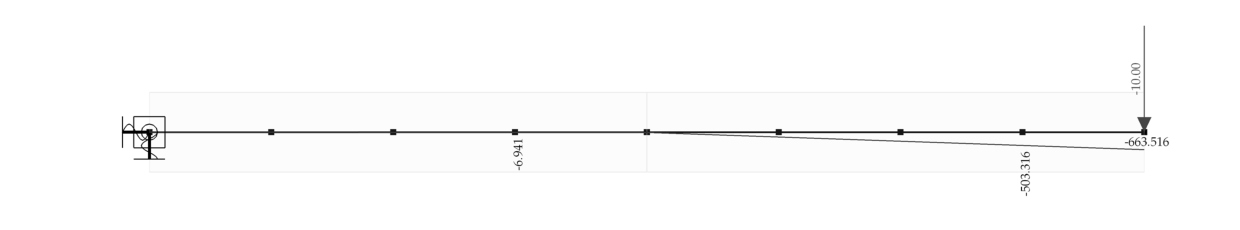
\includegraphics{index_files/mediabag/../imgs/Kragarm_drehfeder_10.pdf}

}

\caption{\label{fig-kragarm-drehfeder-10}Verformungen in \(z\) für
\(F_1\) aus AxisVM mit Drehfedermodell}

\end{figure}%

Das Modell liefert für die erste Laststufe die Gesamtverformung von:

\[
w_{1,tot,F1} = 663.5 \text{mm}
\]

\begin{figure}[H]

\centering{

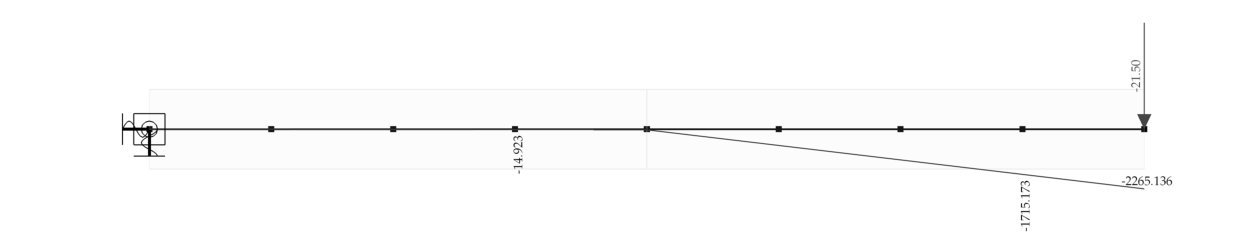
\includegraphics{index_files/mediabag/../imgs/Kragarm_drehfeder_215.pdf}

}

\caption{\label{fig-kragarm-drehfeder-215}Verformungen in \(z\) für
\(F_2\) aus AxisVM mit Drehfedermodell}

\end{figure}%

So wie für die zweite Laststufe folgt die Gesamtverformung zu:

\[
w_{1,tot,F2} = 2265.1 \text{mm}
\]

Das Modell liefert die annähernd gleichen Resultate wie die
Handrechnung. Die Genauigkeit ist zufriedenstellend.

\subsection{Modellierungsalternative
Wegfeder}\label{modellierungsalternative-wegfeder}

Wie bereits in Kapitel~\ref{sec-modellvorstellung} aufgezeigt, lässt
sich das Verhalten der Drehfeder mit einem Wegfederpaar abbilden. Dazu
wird in einem ersten Schritt die Drehfedercharakteristik in eine
Wegfedercharakteristik umgerechnet. Als Grundlage dient die Modellierung
gemäss Abbildung~\ref{fig-verdrehung_verformung}. Die Abbildung zeigt
die kinematische Relation eines reinen Biegeelements.

\begin{figure}[H]

\centering{

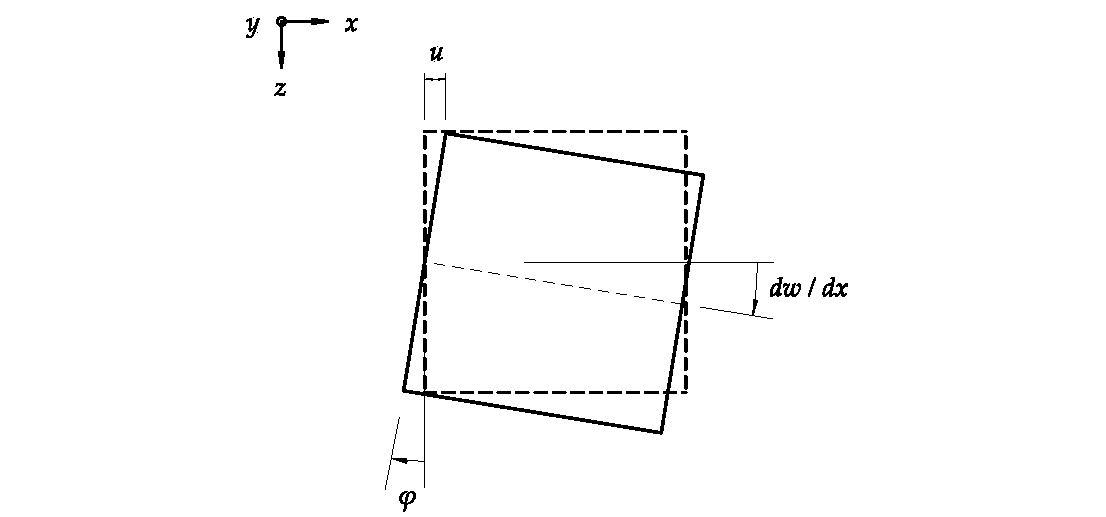
\includegraphics{index_files/mediabag/../imgs/Skizze_Verdrehung_Verformung.pdf}

}

\caption{\label{fig-verdrehung_verformung}Kinematische Relation eines
reinen Biegeelements}

\end{figure}%

Mittels den folgenden Gleichungen lässt sich so die
Wegfedercharakteristik bestimmen. Der Abstand zwischen dem Wegfederpaar
wird mit \(z\) beschrieben.

\[
F = \frac{M}{z}
\]

\[
u = \frac{\tan(\varphi) \cdot z}{2} \simeq \frac{\varphi \cdot z}{2}
\]

Durch die Berücksichtigung der trigonometrischen Funktion ist der
Verlauf nicht exakt bilinear. Eine Approximation mit einem bilinearen
Verlauf führt zu beträchtlichen Abweichungen im Bereich der zweiten
Laststufe \(F_2\). Dies ist auf die geringe Neigung, bzw.
\(k_{\varphi_2}\) der Drehfedercharakteristik im oberen Lastniveau
zurückzuführen.

Die umgerechnete Wegfedercharakteristik ist in
Abbildung~\ref{fig-wegfeder-force} aufgezeigt.

\begin{figure}[H]

\centering{

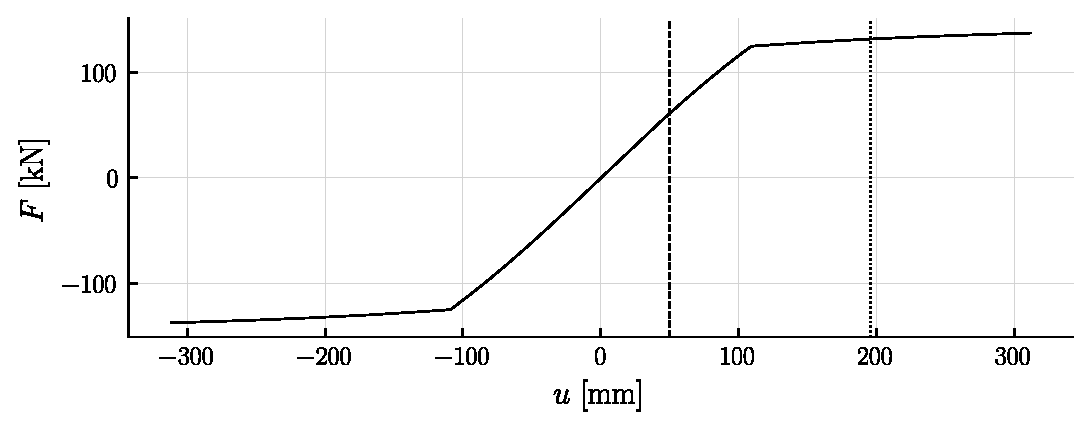
\includegraphics{index_files/mediabag/04_Kragarm_files/figure-pdf/fig-wegfeder-force-output-1.pdf}

}

\caption{\label{fig-wegfeder-force}Charakteristik der Wegfeder}

\end{figure}%

Die Resultate mit dem Modell sind in der Abbildung~\ref{fig-f1-wegfeder}
und Abbildung~\ref{fig-f2-wegfeder} gezeigt.

\begin{figure}[H]

\centering{

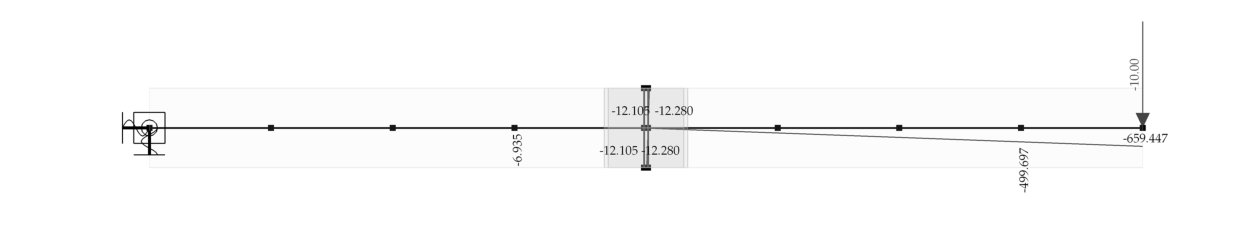
\includegraphics{index_files/mediabag/../imgs/Kragarm_wegfeder_10.pdf}

}

\caption{\label{fig-f1-wegfeder}Verformungen in \(z\) für \(F_1\) aus
AxisVM mit Wegfedermodell}

\end{figure}%

Die maximale Verformung in \(Z\)-Richtung ist für die Laststufe \(1\):

\[
w_{1,tot,F1} = 655 \text{mm}
\]

Und für die Laststufe \(2\):

\[
w_{1,tot,F2} = 2137.8 \text{mm}
\]

Hier zeigt sich eine Abweichung. Diese lässt sich auf die numerisch
approximierte Modellierung der Wegfederbeziehung zurückführen.

\begin{figure}[H]

\centering{

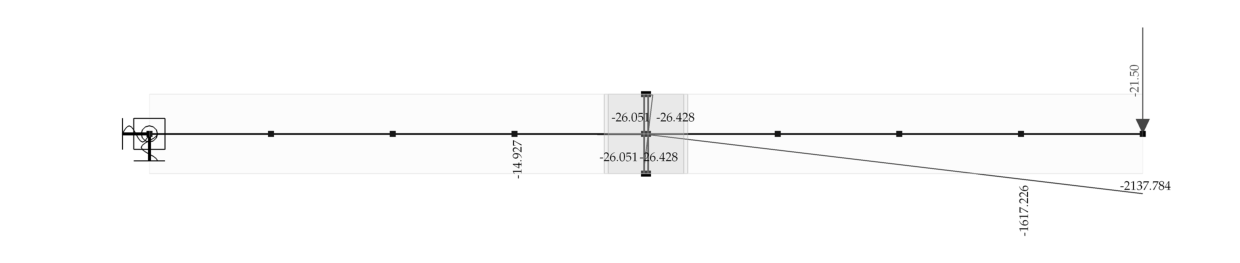
\includegraphics{index_files/mediabag/../imgs/Kragarm_wegfeder_215.pdf}

}

\caption{\label{fig-f2-wegfeder}Verformungen in \(z\) für \(F_2\) aus
AxisVM mit Wegfedermodell}

\end{figure}%

\bookmarksetup{startatroot}

\chapter{Modellverifizierung}\label{modellverifizierung}

In diesem Kapitel werden die beiden Versuche aus der Vorarbeit
{[}\citeproc{ref-gitz_ansatze_2024}{1}{]} mit einem Drehfedermodell,
gemäss dem Beschrieb in Kapitel~\ref{sec-modellvorstellung},
nachgerechnet. Dazu wird eine feine Stabunterteilung gewählt, um das
Verformungsverhalten präzise abzubilden. Detaillierte Berechnungen und
Versuchsbeschriebe, welche als Grundlagen für die Modellierung dienen,
sind in {[}\citeproc{ref-gitz_ansatze_2024}{1}{]} zu finden.
Grundsätzlich gilt, dass für den Betonstahl bilineare
Spannungs-Dehnungs-Beziehungen hinterlegt sind und für den Beton ein
elastisch-ideal-plastisches Gesetz mit Berücksichtigung der
Zugfestigkeit.

\section{Dreipunktbiegeversuch}\label{dreipunktbiegeversuch}

Der Dreipunktbiegeversuch ist der dritte Versuch der Serie A in der
zweiten Versuchsanordnung aus
{[}\citeproc{ref-jager_versuche_2006}{2}{]}, kurz betitelt mit A3V2.
Dieser ist mit einer durchegehenden Längsbewehrung im Zugbereich
bewehrt. Die Schubdübel sind nicht durchgängig verlegt. Dargestellt ist
das Bewehrungslayout in der Abbildung~\ref{fig-bewehrung_a3v2}.

\begin{figure}[H]

\centering{

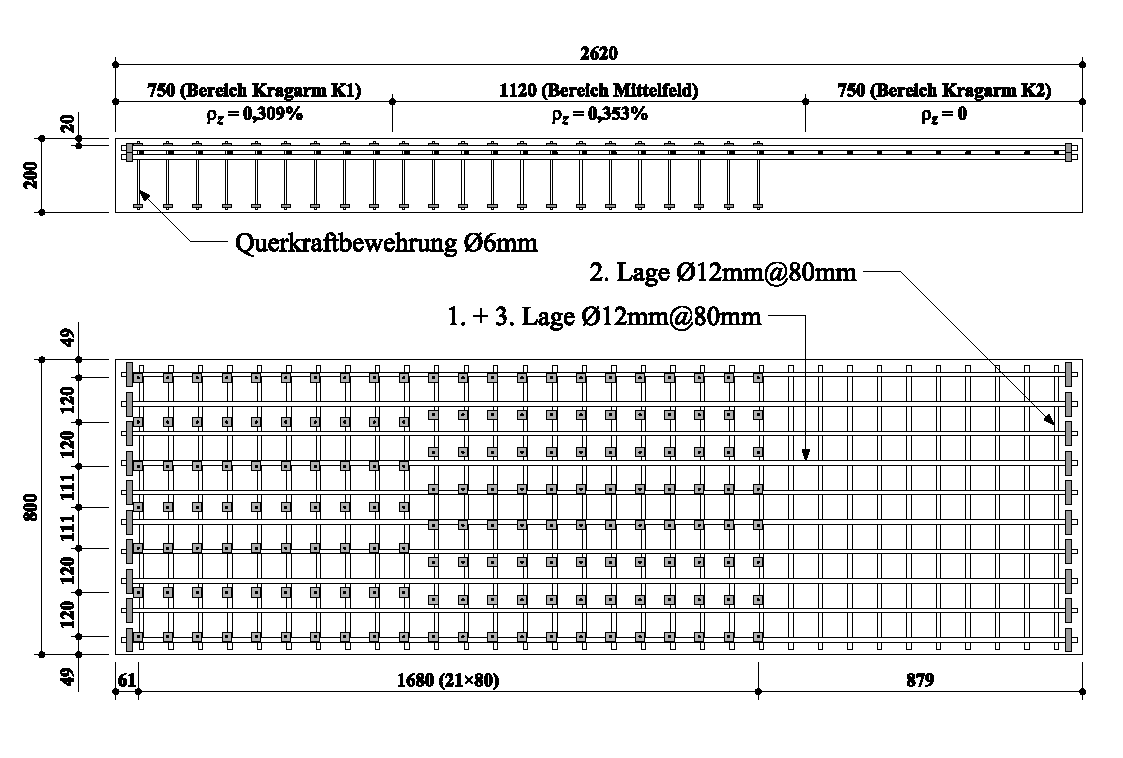
\includegraphics{index_files/mediabag/../imgs/bewehrung_a3v2.pdf}

}

\caption{\label{fig-bewehrung_a3v2}Bewehrunslayout des Versuchs A3V2,
Zeichnung entnommen aus {[}\citeproc{ref-jager_versuche_2006}{2}{]}}

\end{figure}%

Das statische System des Versuchs ist in Abbildung~\ref{fig-system_a3v2}
dargestellt. Das Eigengewicht wird vernachlässigt, da die
Verformungsmessungen nach dem Einbau des Versuchs beginnen, bzw. erst
bei Belastungsbeginn mit der Einzellast.

\begin{figure}[H]

\centering{

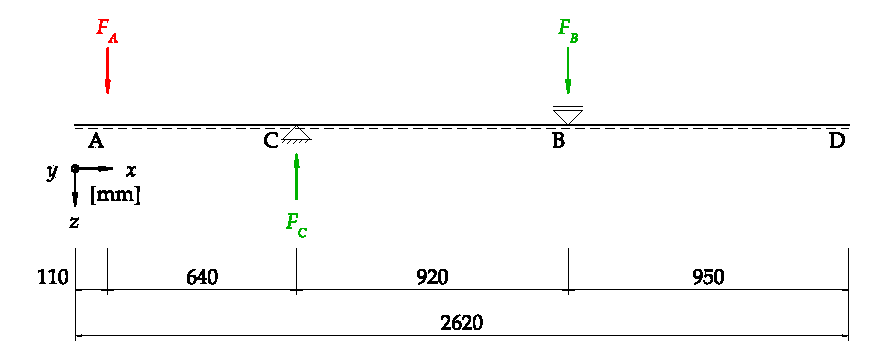
\includegraphics{index_files/mediabag/../imgs/A3V2_system.pdf}

}

\caption{\label{fig-system_a3v2}Statisches System des Versuchs A3V2}

\end{figure}%

Die Abbildung~\ref{fig-qs_a3v2} zeigt den Querschnitt des Versuchs mit
der entsprechenden Bewehrungsführung.

\begin{figure}[H]

\centering{

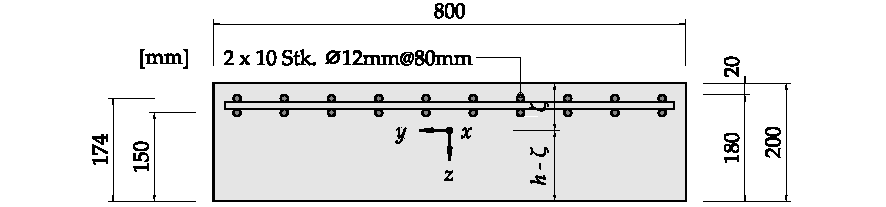
\includegraphics{index_files/mediabag/../imgs/QS_Versuch_A3.pdf}

}

\caption{\label{fig-qs_a3v2}Querschnitt des Versuchs A3V2, Zeichnung
entnommen aus {[}\citeproc{ref-gitz_ansatze_2024}{1}{]}}

\end{figure}%

\subsection{Drehfedercharakteristik}\label{drehfedercharakteristik}

Als erster Eingabeparamter in das Drehfedermodell dient die
Momenten-Krümmungs-Beziehung. Für den Querschnitt ist die nicht-lineare
Beziehung in der Abbildung~\ref{fig-mchi_a3v2} gezeigt. Detaillierte
Berechnungen sind in der Vorarbeit
{[}\citeproc{ref-gitz_ansatze_2024}{1}{]} zu finden.

\begin{figure}[H]

\centering{

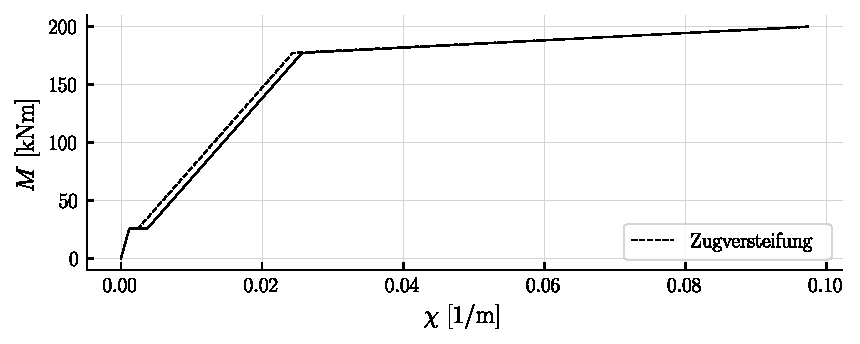
\includegraphics{index_files/mediabag/05_Versuchsnachrechnung_VM1_files/figure-pdf/fig-mchi_a3v2-output-1.pdf}

}

\caption{\label{fig-mchi_a3v2}Momenten-Krümmungs-Beziehung des
Dreipunktbiegeversuchs, übernommen aus
{[}\citeproc{ref-gitz_ansatze_2024}{1}{]}}

\end{figure}%

\subsubsection{Versatzmass}\label{versatzmass}

Ein Ansatz zur Berücksichtigung des Versatzmass ist es ein Versatzmoment
mit dem maximalen Querkraftwiderstand zu bestimmen. Die
Momenten-Krümmungs-Beziehung kann durch diesen Wert vermindert werden
und folglich weicher gestaltet werden.

$$
\begin{aligned}
\theta_{c3_{A3V2}} &= 34.3\ \mathrm{°} \; 
\\[12pt]
V_{Rd_{A3V2}} &= 320.0\ \mathrm{kN} \; 
\\[12pt]
z_{A3V2} &= 140.0\ \mathrm{mm} \; 
\\[12pt]
\Delta_{M_{A3V2}} &= \frac{ V_{Rd_{A3V2}} }{ \tan \left( \theta_{c3_{A3V2}} \right) } \cdot \frac{1} { 2 } \cdot z_{A3V2}  = \frac{ 320.0\ \mathrm{kN} }{ \tan \left( 34.3\ \mathrm{°} \right) } \cdot \frac{1} { 2 } \cdot 140.0\ \mathrm{mm} &= 32.8\ \mathrm{kN} \cdot \mathrm{m}  
\end{aligned}
$$

\begin{figure}[H]

\centering{

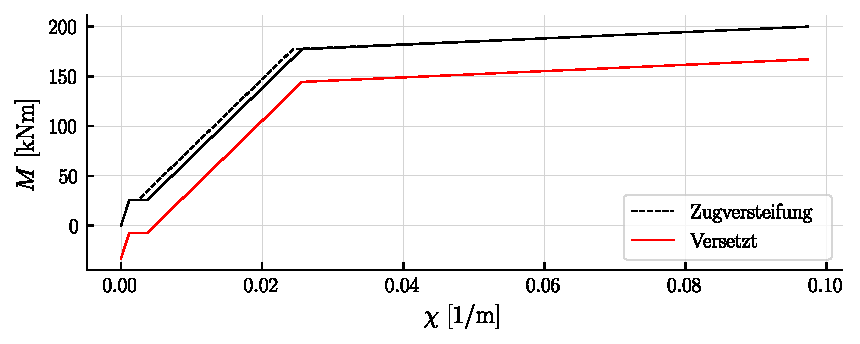
\includegraphics{index_files/mediabag/05_Versuchsnachrechnung_VM1_files/figure-pdf/fig-mchi_a3v2_versatz-output-1.pdf}

}

\caption{\label{fig-mchi_a3v2_versatz}Momenten-Krümmungs-Beziehung des
Dreipunktbiegeversuchs mit Versatzmass}

\end{figure}%

\subsection{Wegfedercharakteristik}\label{wegfedercharakteristik}

\subsubsection{Schiebung}\label{schiebung}

Als Grundlage zur Modellierung der Schubverformungen dient das
Spannungsfeld-Modell in Abbildung~\ref{fig-spannungsfelder_a3v2}. Dabei
wird vorausgesetzt, dass sämtliche Dehnung des Systems in vertikaler
Richtung lediglich aus der Stabdehnung der Schubbewehrung erfolgt. Das
Ziel ist es ein Kraft-Verformungs-Diagramm, bzw. eine
Wegfedercharakteristik zu ermitteln.

\begin{figure}[H]

\centering{

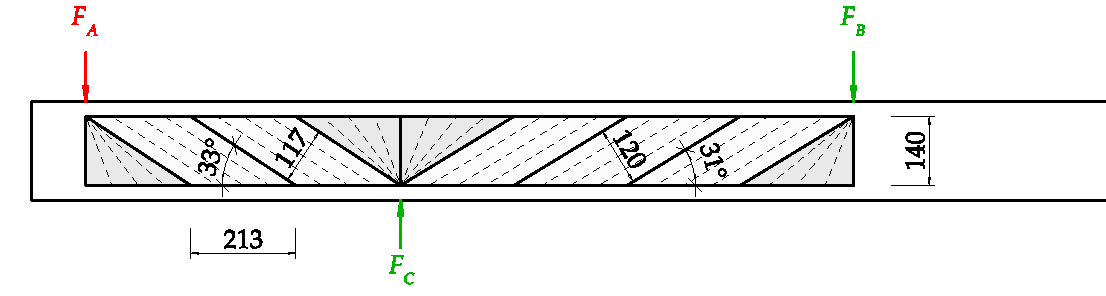
\includegraphics{index_files/mediabag/../imgs/Spannungsfelder_flach.pdf}

}

\caption{\label{fig-spannungsfelder_a3v2}Einteilung in Spannungsfelder
des Versuchs A3V2, Zeichnung entnommen aus
{[}\citeproc{ref-gitz_ansatze_2024}{1}{]}}

\end{figure}%

Durch die Einteilung in Spannungsfelder kann die Anzahl an mitwirkenden
Schubdübeln bestimmt werden. Mit der Querschnittsfläche der mitwirkenden
Dübel kann das nicht-lineare Spannungs-Dehnungs-Verhalten in ein
Kraft-Verformungs-Diagramm bzw. in eine Wegfedercharakteristik
umgewandelt werden. Die bekannte Dehnung aus der Stahlkennlinie wird
über den Hebelarm der inneren Kräfte zu einer Verformung umgewandelt.
Wichtig dabei ist die Elementlänge der biegesteifen Stäbe im FEM-Modell.
Dazu wird die Verformung um den Faktor gemäss der folgenden Gleichung
reduziert, bzw. die Steifigkeit der Feder um diesen Faktor erhöht.

\[
\gamma_{E} = \frac{z \cdot \cot(\theta)}{n_{E}}
\]

\(n_{E}\) steht für die Anzahl steifer Stabelemente

\begin{figure}[H]

\centering{

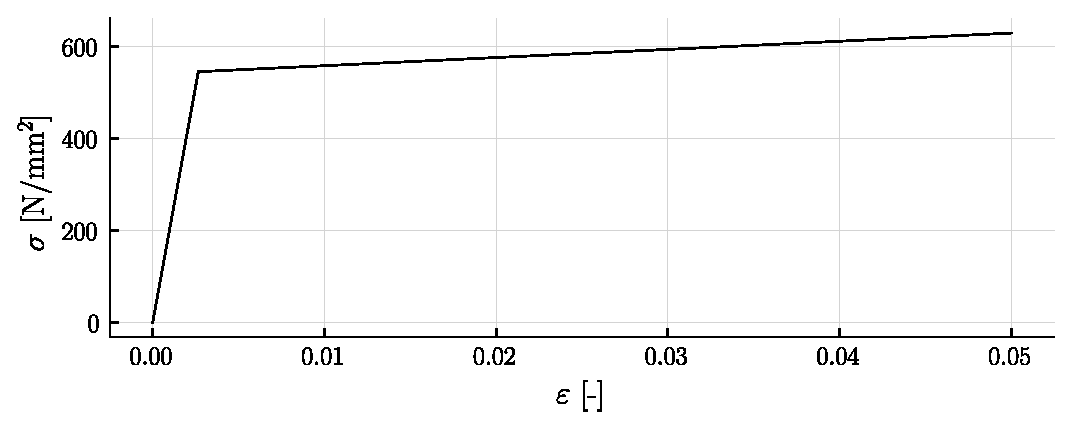
\includegraphics{index_files/mediabag/05_Versuchsnachrechnung_VM1_files/figure-pdf/fig-sigma-eps-a3v2-output-1.pdf}

}

\caption{\label{fig-sigma-eps-a3v2}Spannungs-Dehnungs-Beziehung der
Schubbewehrung, übernommen aus
{[}\citeproc{ref-gitz_ansatze_2024}{1}{]}}

\end{figure}%

Folgend sind die Parameter zur Bestimmung der Wegfedercharakteristik in
vertikaler Richtung gezeigt. Der gewählte Neigungswinkel der
Spannungsfelder \(/theta_{c3}\) gilt grundsätzlich nur im Bruchzustand.
Als Approximation wird die daraus bestimmte Wegfedercharakteristik für
sämtliche Laststufen angesetzt. Dies führt zu Abweichungen im Lastniveau
unterhalb der Traglast, sofern die Schubverformung einen signifikanten
Einfluss an der der Gesamtverformung liefern.

$$
\begin{aligned}
\oslash_{sw_{A3V2}} &= 6.0\ \mathrm{mm} \; 
 &S_{sw_{A3V2}} &= 80.0\ \mathrm{mm} \; 
 &b_{w_{A3V2}} &= 800.0\ \mathrm{mm} \; 
\\[12pt]
 E_{sw_{A3V2}} &= 205000.0\ \frac{\mathrm{N}}{\mathrm{mm}^{2}} \; 
 &E_{sh_{A3V2}} &= 1774.5\ \frac{\mathrm{N}}{\mathrm{mm}^{2}} \;
\end{aligned}
$$

Die Querschnittsfläche der Schubbewehrung und der Bewehrungsgehalt
bestimmt sich zu:

$$
\begin{aligned}
A_{sw_{A3V2}} &= 7 \cdot \left( \frac{ \oslash_{sw_{A3V2}} }{ 2 } \right) ^{ 2 } \cdot \pi  = 7 \cdot \left( \frac{ 6.00\ \mathrm{mm} }{ 2 } \right) ^{ 2 } \cdot 3.14 &= 197.92\ \mathrm{mm}^{2}  
\\[12pt]
a_{sw_{A3V2}} &= A_{sw_{A3V2}} \cdot \frac{ 1000 \cdot \mathrm{mm} }{ S_{sw_{A3V2}} } \cdot \frac{1} { m }  = 197.92\ \mathrm{mm}^{2} \cdot \frac{ 1000 \cdot \mathrm{mm} }{ 80.00\ \mathrm{mm} } \cdot \frac{1} { \mathrm{m} } &= 2474.00\ \frac{\mathrm{mm}^{2}}{\mathrm{m}}  
\\[12pt]
\rho_{sw_{A3V2}} &= \left( \frac{ a_{sw_{A3V2}} }{ b_{w_{A3V2}} } \right)  = \left( \frac{ 2474.00\ \frac{\mathrm{mm}^{2}}{\mathrm{m}} }{ 800.00\ \mathrm{mm} } \right) &= 0.31\ \mathrm{\%}  
\end{aligned}
$$

Der Reduktionsfaktor bestimmt sich zu:

$$
\begin{aligned}
\gamma_{E_{A3V2}} &= z_{A3V2} \cdot \frac{ 1 }{ \tan \left( \theta_{c3_{A3V2}} \right) } \cdot \frac{1} { l_{element} } \; 
\end{aligned}
$$

$$
\begin{aligned}
\gamma_{E_{A3V2}} &= 21\ \;
\end{aligned}
$$

Die Abbildung~\ref{fig-wegfeder-schub-a3v2} zeigt das
Kraft-Verformungs-Verhalten für die Gelenke des Stabmodells in
vertikaler Richtung.

\begin{figure}[H]

\centering{

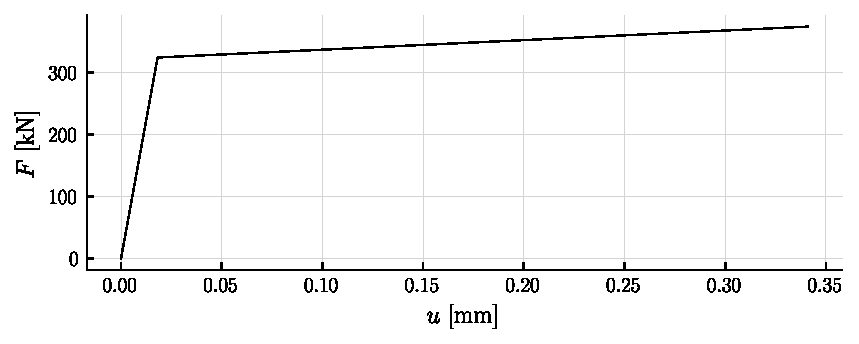
\includegraphics{index_files/mediabag/05_Versuchsnachrechnung_VM1_files/figure-pdf/fig-wegfeder-schub-a3v2-output-1.pdf}

}

\caption{\label{fig-wegfeder-schub-a3v2}Berechnete
Wegfedercharakteristik des Schubgelenks vom Versuch A3V2}

\end{figure}%

\subsection{Versuchsvergleich}\label{versuchsvergleich}

Mit den bestimmten Federcharakteristiken kann die Biegelinie des Systems
ermittelt werden unter Berücksichtigung der Schub- und Biegeverformungen
auf nicht-linearen Grundlagen. Die Abbildung~\ref{fig-fwa3v2} zeigt das
Last-Verformungs-Diagramm des Systems am Punkt \(w_1\). Das Modell
beschreibt den Verformungsverlauf zufriedenstellend.

\begin{figure}[H]

\centering{

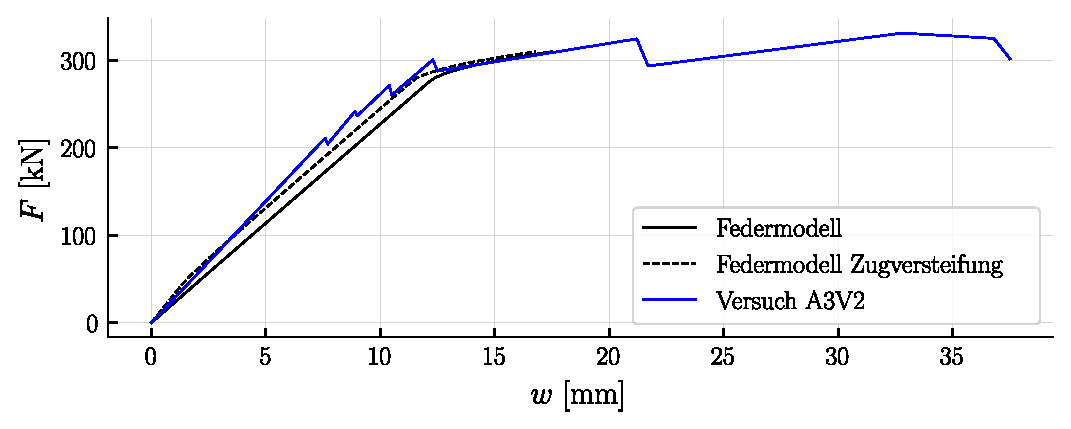
\includegraphics{index_files/mediabag/05_Versuchsnachrechnung_VM1_files/figure-pdf/fig-fwa3v2-output-1.pdf}

}

\caption{\label{fig-fwa3v2}Last-Verformungs-Verlauf am Punkt \(w_1\) mit
dem Federmodell und den Versuchsmessungen}

\end{figure}%

Der Verdrehungsverlauf in Abbildung~\ref{fig-phi-max-a3v2} lässt sich
ebenfalls direkt aus dem Modell exportieren. Durch die Ableitung des
Verlaufs resultiert der Krümmungsverlauf, dargestellt in
Abbildung~\ref{fig-chi-max-a3v2}.

\begin{figure}[H]

\centering{

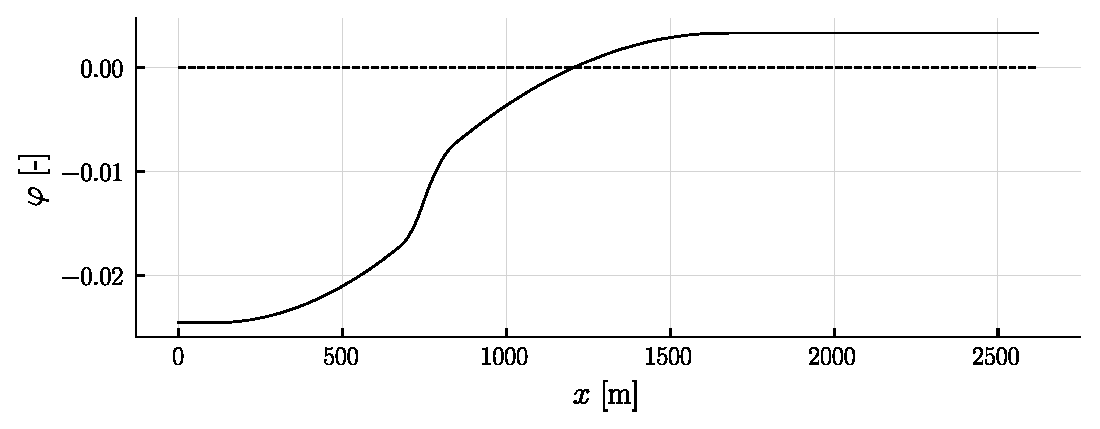
\includegraphics{index_files/mediabag/05_Versuchsnachrechnung_VM1_files/figure-pdf/fig-phi-max-a3v2-output-1.pdf}

}

\caption{\label{fig-phi-max-a3v2}Verdrehungsverlauf aus dem Federmodell
für die Höchstlast}

\end{figure}%

Der Krümmungsverlauf gibt Aufschluss über den Fliessbereich der
Bewehrung, bzw. über den Steifigkeitenverlauf entlang der Stabachse.

\begin{figure}[H]

\centering{

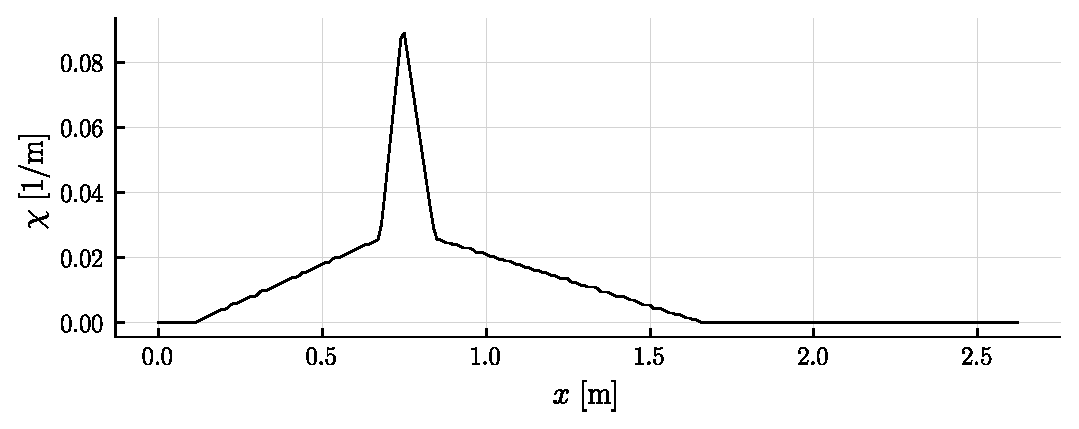
\includegraphics{index_files/mediabag/05_Versuchsnachrechnung_VM1_files/figure-pdf/fig-chi-max-a3v2-output-1.pdf}

}

\caption{\label{fig-chi-max-a3v2}Berechneter Krümmungsverlauf aus dem
Verdrehungsverlauf}

\end{figure}%

\newpage{}

\section{Vierpunktbiegeversuch}\label{vierpunktbiegeversuch}

Der Vierpunktbiegeversuch ist aus dem Paper
{[}\citeproc{ref-tue_einfluss_2019}{3}{]} entnommen. Auffallend bei
diesem Versuch ist die niedrig gehaltene Schubbewehrung. Dazu sind in
Längsrichtung Stäbe mit unterschiedlicher Güte verlegt.

\begin{figure}[H]

\centering{

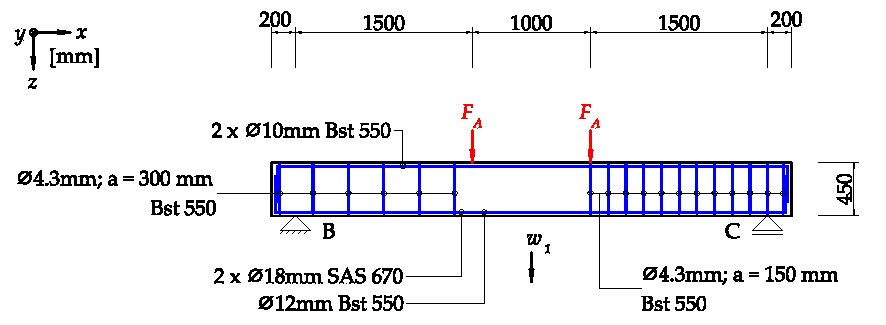
\includegraphics{index_files/mediabag/../imgs/versuchsskizze_14.pdf}

}

\caption{\label{fig-versuchsskizze-SV14}Bewehrungslayout des Versuchs
SV14, Zeichnung entnommen aus {[}\citeproc{ref-gitz_ansatze_2024}{1}{]}}

\end{figure}%

Der Querschnitt ist in der Abbildung~\ref{fig-QS-SV14} gezeigt. Die
Druckbewehrung wird vernachlässigt.

\begin{figure}[H]

\centering{

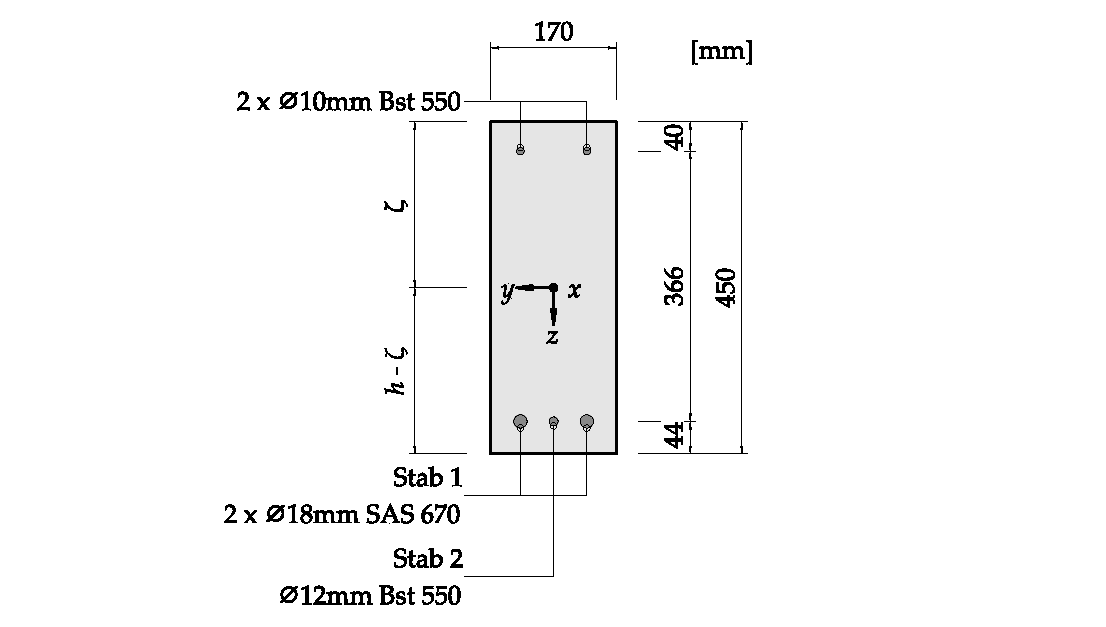
\includegraphics{index_files/mediabag/../imgs/QS_Versuch14.pdf}

}

\caption{\label{fig-QS-SV14}Querschnitt des Versuchs SV14, Zeichnung
entnommen aus {[}\citeproc{ref-gitz_ansatze_2024}{1}{]}}

\end{figure}%

Das statische System ist in der Abbildung~\ref{fig-system-SV14} gezeigt.
Auch hier wird das Eigengewicht, wie im Versuch A3V2, vernachlässigt.
Die gemessene und rechnerisch bestimmte Verformung gelten für den
Mittelspunkt, beschrieben mit \(w_1\).

\begin{figure}[H]

\centering{

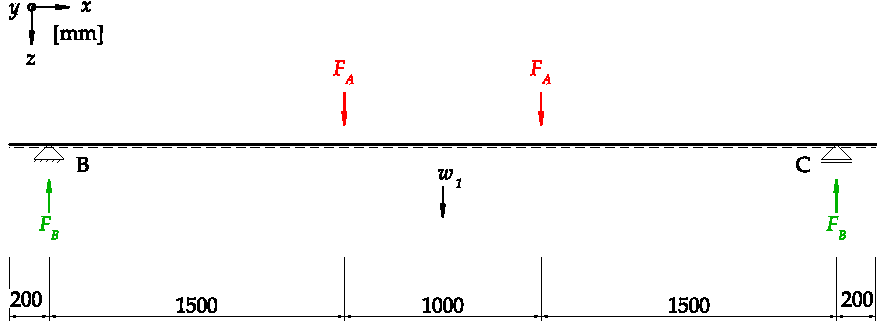
\includegraphics{index_files/mediabag/../imgs/statisches_system_14.pdf}

}

\caption{\label{fig-system-SV14}Statisches System des Versuchs SV14,
Zeichnung entnommen aus {[}\citeproc{ref-gitz_ansatze_2024}{1}{]}}

\end{figure}%

\subsection{Drehfedercharakteristik}\label{drehfedercharakteristik-1}

Als Grundlage für die Drehfedercharakteristik gilt die
Momenten-Krümmungs-Beziehung. Für den Querschnitt des Versuchs SV14 gilt
die Beziehung gemäss Abbildung~\ref{fig-mchi_sv14}. Für detaillierte
Berechnungen ist die Vorarbeit {[}\citeproc{ref-gitz_ansatze_2024}{1}{]}
zu konsultieren.

\begin{figure}[H]

\centering{

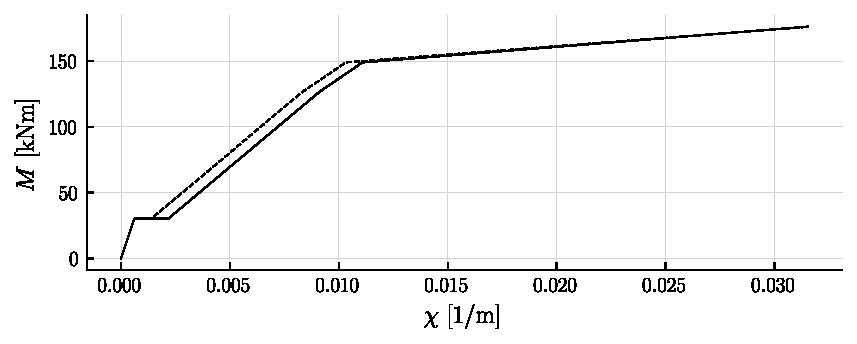
\includegraphics{index_files/mediabag/05_Versuchsnachrechnung_VM1_files/figure-pdf/fig-mchi_sv14-output-1.pdf}

}

\caption{\label{fig-mchi_sv14}Momenten-Krümmungs-Beziehung des
Vierpunktbiegeversuchs, übernommen aus
{[}\citeproc{ref-gitz_ansatze_2024}{1}{]}}

\end{figure}%

\subsection{Versatzmass}\label{versatzmass-1}

Das Versatzmass gilt es noch zu bestimmen:

$$
\begin{aligned}
V_{Rd_{SV14}} &= 105.0\ \mathrm{kN} \; 
\\[12pt]
z_{SV14} &= 359.0\ \mathrm{mm} \; 
\\[12pt]
\theta_{c3_{SV14}} &= 12.3\ \mathrm{°} \; 
\\[12pt]
\Delta_{M_{SV14}} &= \frac{ V_{Rd_{SV14}} }{ \tan \left( \theta_{c3_{SV14}} \right) } \cdot \frac{1} { 2 } \cdot z_{SV14}  = \frac{ 105.0\ \mathrm{kN} }{ \tan \left( 12.3\ \mathrm{°} \right) } \cdot \frac{1} { 2 } \cdot 359.0\ \mathrm{mm} &= 86.4\ \mathrm{kN} \cdot \mathrm{m}  
\end{aligned}
$$

\begin{figure}[H]

\centering{

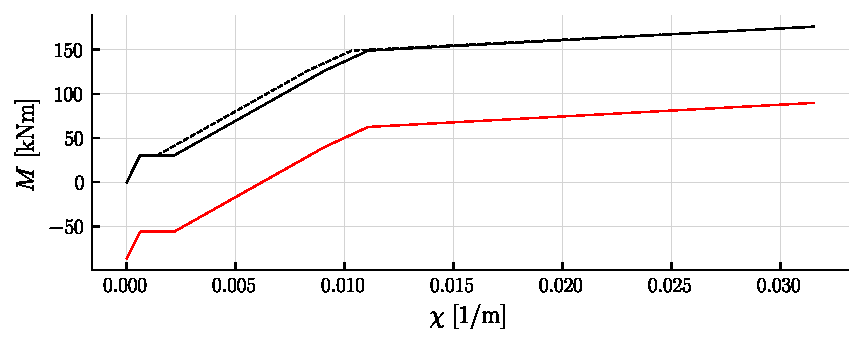
\includegraphics{index_files/mediabag/05_Versuchsnachrechnung_VM1_files/figure-pdf/fig-mchi_sv14_versatz-output-1.pdf}

}

\caption{\label{fig-mchi_sv14_versatz}Momenten-Krümmungs-Beziehung des
Vierpunktbiegeversuchs mit Versatzmass}

\end{figure}%

\subsection{Wegfedercharakteristik}\label{wegfedercharakteristik-1}

\subsubsection{Schiebung}\label{schiebung-1}

Die Wegfedercharakteristik basiert auf der Spannungsfeldmodellierung
gemäss der Abbildung~\ref{fig-spannungsfelder_sv14}

\begin{figure}[H]

\centering{

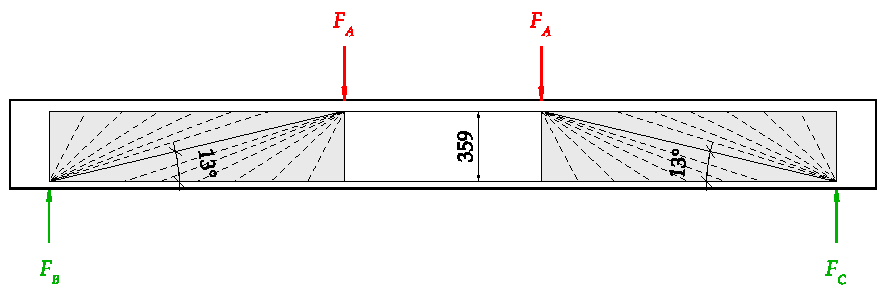
\includegraphics{index_files/mediabag/../imgs/spannungsfelder_sv14.pdf}

}

\caption{\label{fig-spannungsfelder_sv14}Einteilung in Spannungsfelder
des Versuchs SV14, Zeichnung entnommen aus
{[}\citeproc{ref-gitz_ansatze_2024}{1}{]}}

\end{figure}%

Die Einteilung in Spannungsfelder ermöglicht die Bestimmung der
mitwirkenden Schubbewehrung beim Versagen des Querschnitts. Die Neigung
des Feldes ist so gewählt damit der Querkraftwiderstand der
Schubbewehrung der Traglast des Systems entspricht.

\begin{figure}[H]

\centering{

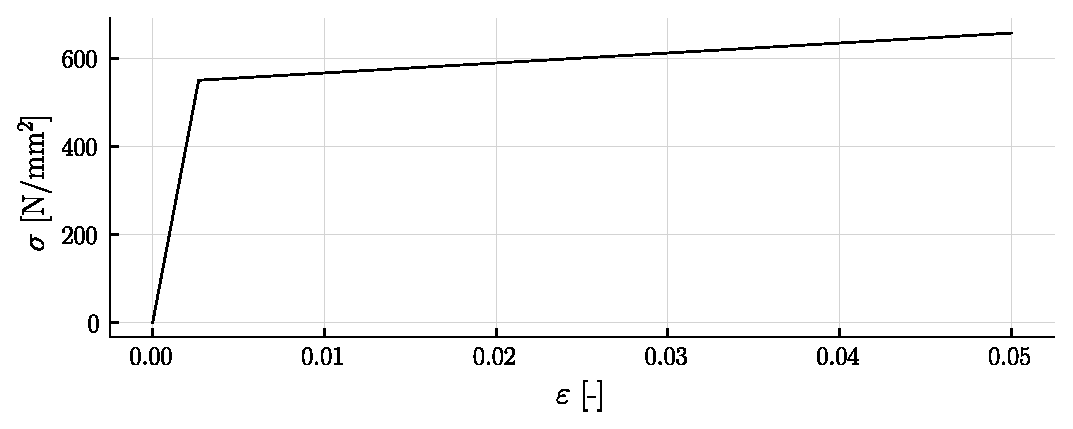
\includegraphics{index_files/mediabag/05_Versuchsnachrechnung_VM1_files/figure-pdf/fig-sigma-epsilon-sv14-output-1.pdf}

}

\caption{\label{fig-sigma-epsilon-sv14}Spannungs-Dehnungs-Beziehung der
Schubbewehrung, übernommen aus
{[}\citeproc{ref-gitz_ansatze_2024}{1}{]}}

\end{figure}%

Folgend sind die Parameter zur Bestimmung der Wegfedercharakteristik in
vertikaler Richtung gezeigt.

$$
\begin{aligned}
\oslash_{sw_{SV14}} &= 4.3\ \mathrm{mm} \; 
 &b_{w_{SV14}} &= 170.0\ \mathrm{mm} \; 
 &S_{sw_{SV14}} &= 300.0\ \mathrm{mm} \; 
\\[12pt]
 E_{sw_{SV14}} &= 205000.0\ \frac{\mathrm{N}}{\mathrm{mm}^{2}} \; 
 &E_{sh_{SV14}} &= 2261.3\ \frac{\mathrm{N}}{\mathrm{mm}^{2}} \;
\end{aligned}
$$

Die Querschnittsfläche der Schubbewehrung und der Bewehrungsgehalt
bestimmt sich zu:

$$
\begin{aligned}
A_{sw} &= 2 \cdot \left( \frac{ \oslash_{sw_{SV14}} }{ 2 } \right) ^{ 2 } \cdot \pi  = 2 \cdot \left( \frac{ 4.30\ \mathrm{mm} }{ 2 } \right) ^{ 2 } \cdot 3.14 &= 29.04\ \mathrm{mm}^{2}  
\\[12pt]
a_{sw_{SV14}} &= A_{sw} \cdot 1000 \cdot \frac{ \mathrm{mm} }{ S_{sw_{SV14}} } \cdot \frac{1} { m }  = 29.04\ \mathrm{mm}^{2} \cdot 1000 \cdot \frac{ \mathrm{mm} }{ 300.00\ \mathrm{mm} } \cdot \frac{1} { \mathrm{m} } &= 96.81\ \frac{\mathrm{mm}^{2}}{\mathrm{m}}  
\\[12pt]
\rho_{sw_{SV14}} &= \left( \frac{ a_{sw_{SV14}} }{ b_{w_{SV14}} } \right)  = \left( \frac{ 96.81\ \frac{\mathrm{mm}^{2}}{\mathrm{m}} }{ 170.00\ \mathrm{mm} } \right) &= 0.06\ \mathrm{\%}  
\end{aligned}
$$

Der Reduktionsfaktor bestimmt sich zu:

$$
\begin{aligned}
\gamma_{E_{SV14}} &= \left( z_{SV14} \cdot \frac{ 1 }{ \tan \left( \theta_{c3_{SV14}} \right) } \cdot \frac{1} { l_{element} } \right) \; 
\end{aligned}
$$

$$
\begin{aligned}
\gamma_{E_{SV14}} &= 165\ \;
\end{aligned}
$$

Die Abbildung~\ref{fig-wegfeder-schub-sv14} zeigt das
Kraft-Verformungs-Verhalten für die Gelenke des Stabmodells in
vertikaler Richtung.

\begin{figure}[H]

\centering{

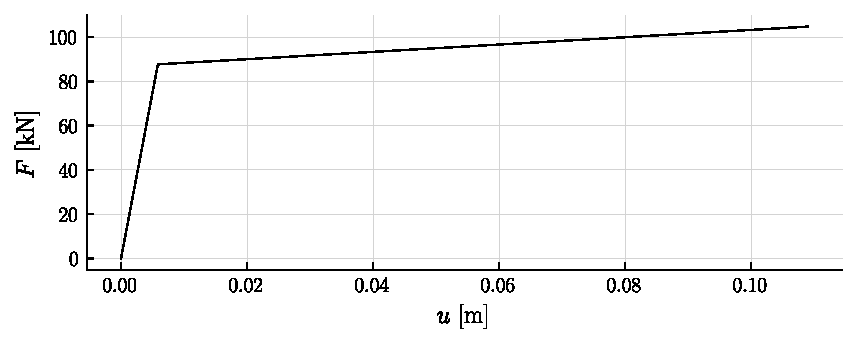
\includegraphics{index_files/mediabag/05_Versuchsnachrechnung_VM1_files/figure-pdf/fig-wegfeder-schub-sv14-output-1.pdf}

}

\caption{\label{fig-wegfeder-schub-sv14}Berechnete
Wegfedercharakteristik des Schubgelenks vom Versuch SV14}

\end{figure}%

\subsection{Versuchsvergleich}\label{versuchsvergleich-1}

Mit den bestimmten Federcharakteristiken kann die Biegelinie des Systems
ermittelt werden unter Berücksichtigung der Schub- und Biegeverformungen
auf nicht-linearen Grundlagen. Die Abbildung~\ref{fig-l-w-sv14} zeigt
das Last-Verformungs-Diagramm des Systems am Punkt \(w_1\). Der
Verformungsverlauf zeigt Abweichungen zu den gemessenen Resultate. Dies
ist auf das Unterschlagen der Längszugkraft aus Querkraft
zurückzuführen.

\begin{figure}[H]

\centering{

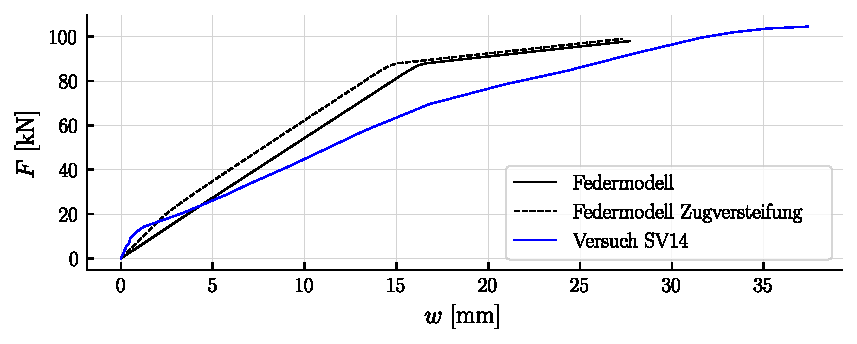
\includegraphics{index_files/mediabag/05_Versuchsnachrechnung_VM1_files/figure-pdf/fig-l-w-sv14-output-1.pdf}

}

\caption{\label{fig-l-w-sv14}Last-Verformungs-Verlauf am Punkt \(w_1\),
für das Federmodell und den Versuch}

\end{figure}%

\bookmarksetup{startatroot}

\chapter{Versuch mit Vorspannung}\label{versuch-mit-vorspannung}

\section{Parameter}\label{parameter}

$$
\begin{aligned}
A_{p} &= 140.0\ \mathrm{mm}^{2} \; \;\textrm{(pro Litze)}
 &n_{l} &= 3 \; \;\textrm{(Litzen in Spannglied)}
 &n_{x} &= 2 \; \;\textrm{(Spannglieder)}
\\[12pt]
 f_{p01} &= 1729.0\ \mathrm{MPa} \; 
 &f_{p02} &= 1764.0\ \mathrm{MPa} \; 
 &E_{P} &= 190000.0\ \mathrm{MPa} \; 
\\[12pt]
 P_{t0} &= 335.0\ \mathrm{kN} \; \;\textrm{(pro Spannglied)}
\end{aligned}
$$

$$
\begin{aligned}
\kappa &= \left( \frac{ P_{t0} }{ n_{l} \cdot A_{p} \cdot f_{p01} } \right)  = \left( \frac{ 335.0\ \mathrm{kN} }{ 3 \cdot 140.0\ \mathrm{mm}^{2} \cdot 1729.0\ \mathrm{MPa} } \right) &= 0.5\  
\end{aligned}
$$

\section{Momenten-Krümmungs-Beziehung}\label{momenten-kruxfcmmungs-beziehung}

\bookmarksetup{startatroot}

\chapter*{Literatur}\label{literatur}
\addcontentsline{toc}{chapter}{Literatur}

\markboth{Literatur}{Literatur}

\phantomsection\label{refs}
\begin{CSLReferences}{0}{1}
\bibitem[\citeproctext]{ref-gitz_ansatze_2024}
\CSLLeftMargin{1. }%
\CSLRightInline{Gitz P (2024) Ansätze zur {Verformungsberechnung}. HSLU
Technik \& Architektur}

\bibitem[\citeproctext]{ref-jager_versuche_2006}
\CSLLeftMargin{2. }%
\CSLRightInline{Jäger T, Marti P (2006) Versuche zum
{Querkraftwiderstand} und zum {Verformungsvermögen} von
{Stahlbetonplatten}. IBK Bericht 294.
\url{https://doi.org/10.3929/ethz-a-005195576}}

\bibitem[\citeproctext]{ref-tue_einfluss_2019}
\CSLLeftMargin{3. }%
\CSLRightInline{Tue NV, Ehmann R, Betschoga C, Tung ND (2019) Einfluss
geringer {Querkraftbewehrung} auf die {Querkrafttragfähigkeit} von
{Stahlbetonbalken} unterschiedlicher {M}/{V}-{Kombinationen}. Beton- und
Stahlbetonbau 114(4):217--230.
https://doi.org/\url{https://doi.org/10.1002/best.201800075}}

\end{CSLReferences}



\end{document}
